
\documentclass[11pt]{article}
\usepackage[utf8]{inputenc}
\usepackage{amsmath,amsthm,amsfonts,amssymb,amscd}
\usepackage{multirow,booktabs}
\usepackage[table]{xcolor}
\usepackage{fullpage}
\usepackage{lastpage}
\usepackage{enumitem}
\usepackage{fancyhdr}
\usepackage{mathrsfs}
\usepackage{wrapfig}
\usepackage{setspace}
\usepackage{calc}
\usepackage{multicol}
\usepackage{cancel}
\usepackage[retainorgcmds]{IEEEtrantools}
\usepackage[margin=3cm]{geometry}
\usepackage{amsmath}
\newlength{\tabcont}
\setlength{\parindent}{0.0in}
\setlength{\parskip}{0.05in}
\usepackage{empheq}
\usepackage{framed}
\usepackage[most]{tcolorbox}
\usepackage{xcolor}
\colorlet{shadecolor}{orange!15}
\parindent 0in
\parskip 12pt
\geometry{margin=1in, headsep=0.25in}
\theoremstyle{definition}
\newtheorem{defn}{Definition}
\newtheorem{reg}{Rule}
\newtheorem{exer}{Exercise}
\newtheorem{note}{Note}

\usepackage[superscript,biblabel]{cite}
\usepackage{hyperref}
\hypersetup{colorlinks,linkcolor={blue},citecolor={blue},urlcolor={orange}}

\usepackage{graphicx}
%Path relative to the main .tex file
\graphicspath{ {./images/} }

\title{\textbf{Heart rate variability analyzer}}
\author{
  Russel Shawn Dsouza\\
  171EC143
  \and
  Sathvik S Prabhu\\
  171EC146
}
\date{13 November, 2019}


\begin{document}
  \maketitle
  \thispagestyle{empty}
  % TODO Change titlepage to add logo

  \newpage
  \tableofcontents
  \thispagestyle{empty}

  \setcounter{page}{1}
  \newpage
  \section{Introduction}
<<<<<<< HEAD
  
=======
  The study and analysis of short-term and long-term variability in heart rate reflects the functioning of the vagal nerve and the sympathetic function of the autonomic nervous system, respectively.
  Heart rate variability can therefore be not only used as a monitoring tool in the diagnosis of cardiac ailments but also in clinical conditions with altered autonomic nervous system function.
  n diabetic patients, low heart rate variability is associated with an increased risk for sudden cardiac death.
  In neurologic disorders such as brain damage, the Guillain-Barre syndrome and uremic neuropathy, heart rate variability analysis can provide insight into which division of the autonomic nervous system is most affected.
  The analysis of the effects of drugs can also be studied using heart rate variability as it can also shed light on the mode of action of drugs.

  A typical ECG signal is characterized by a P wave, a QRS complex consisting of Q,R and S waves and a T wave as shown in figure \ref{fig:pqrst}.
  The automatic detection of the QRS complex or the R peaks in a long term electrocardiogram (ECG) signal is one of the most important steps in the diagnosis of cardiac disorders, biometric and ECG coding systems.

  \begin{figure}
    \centering
    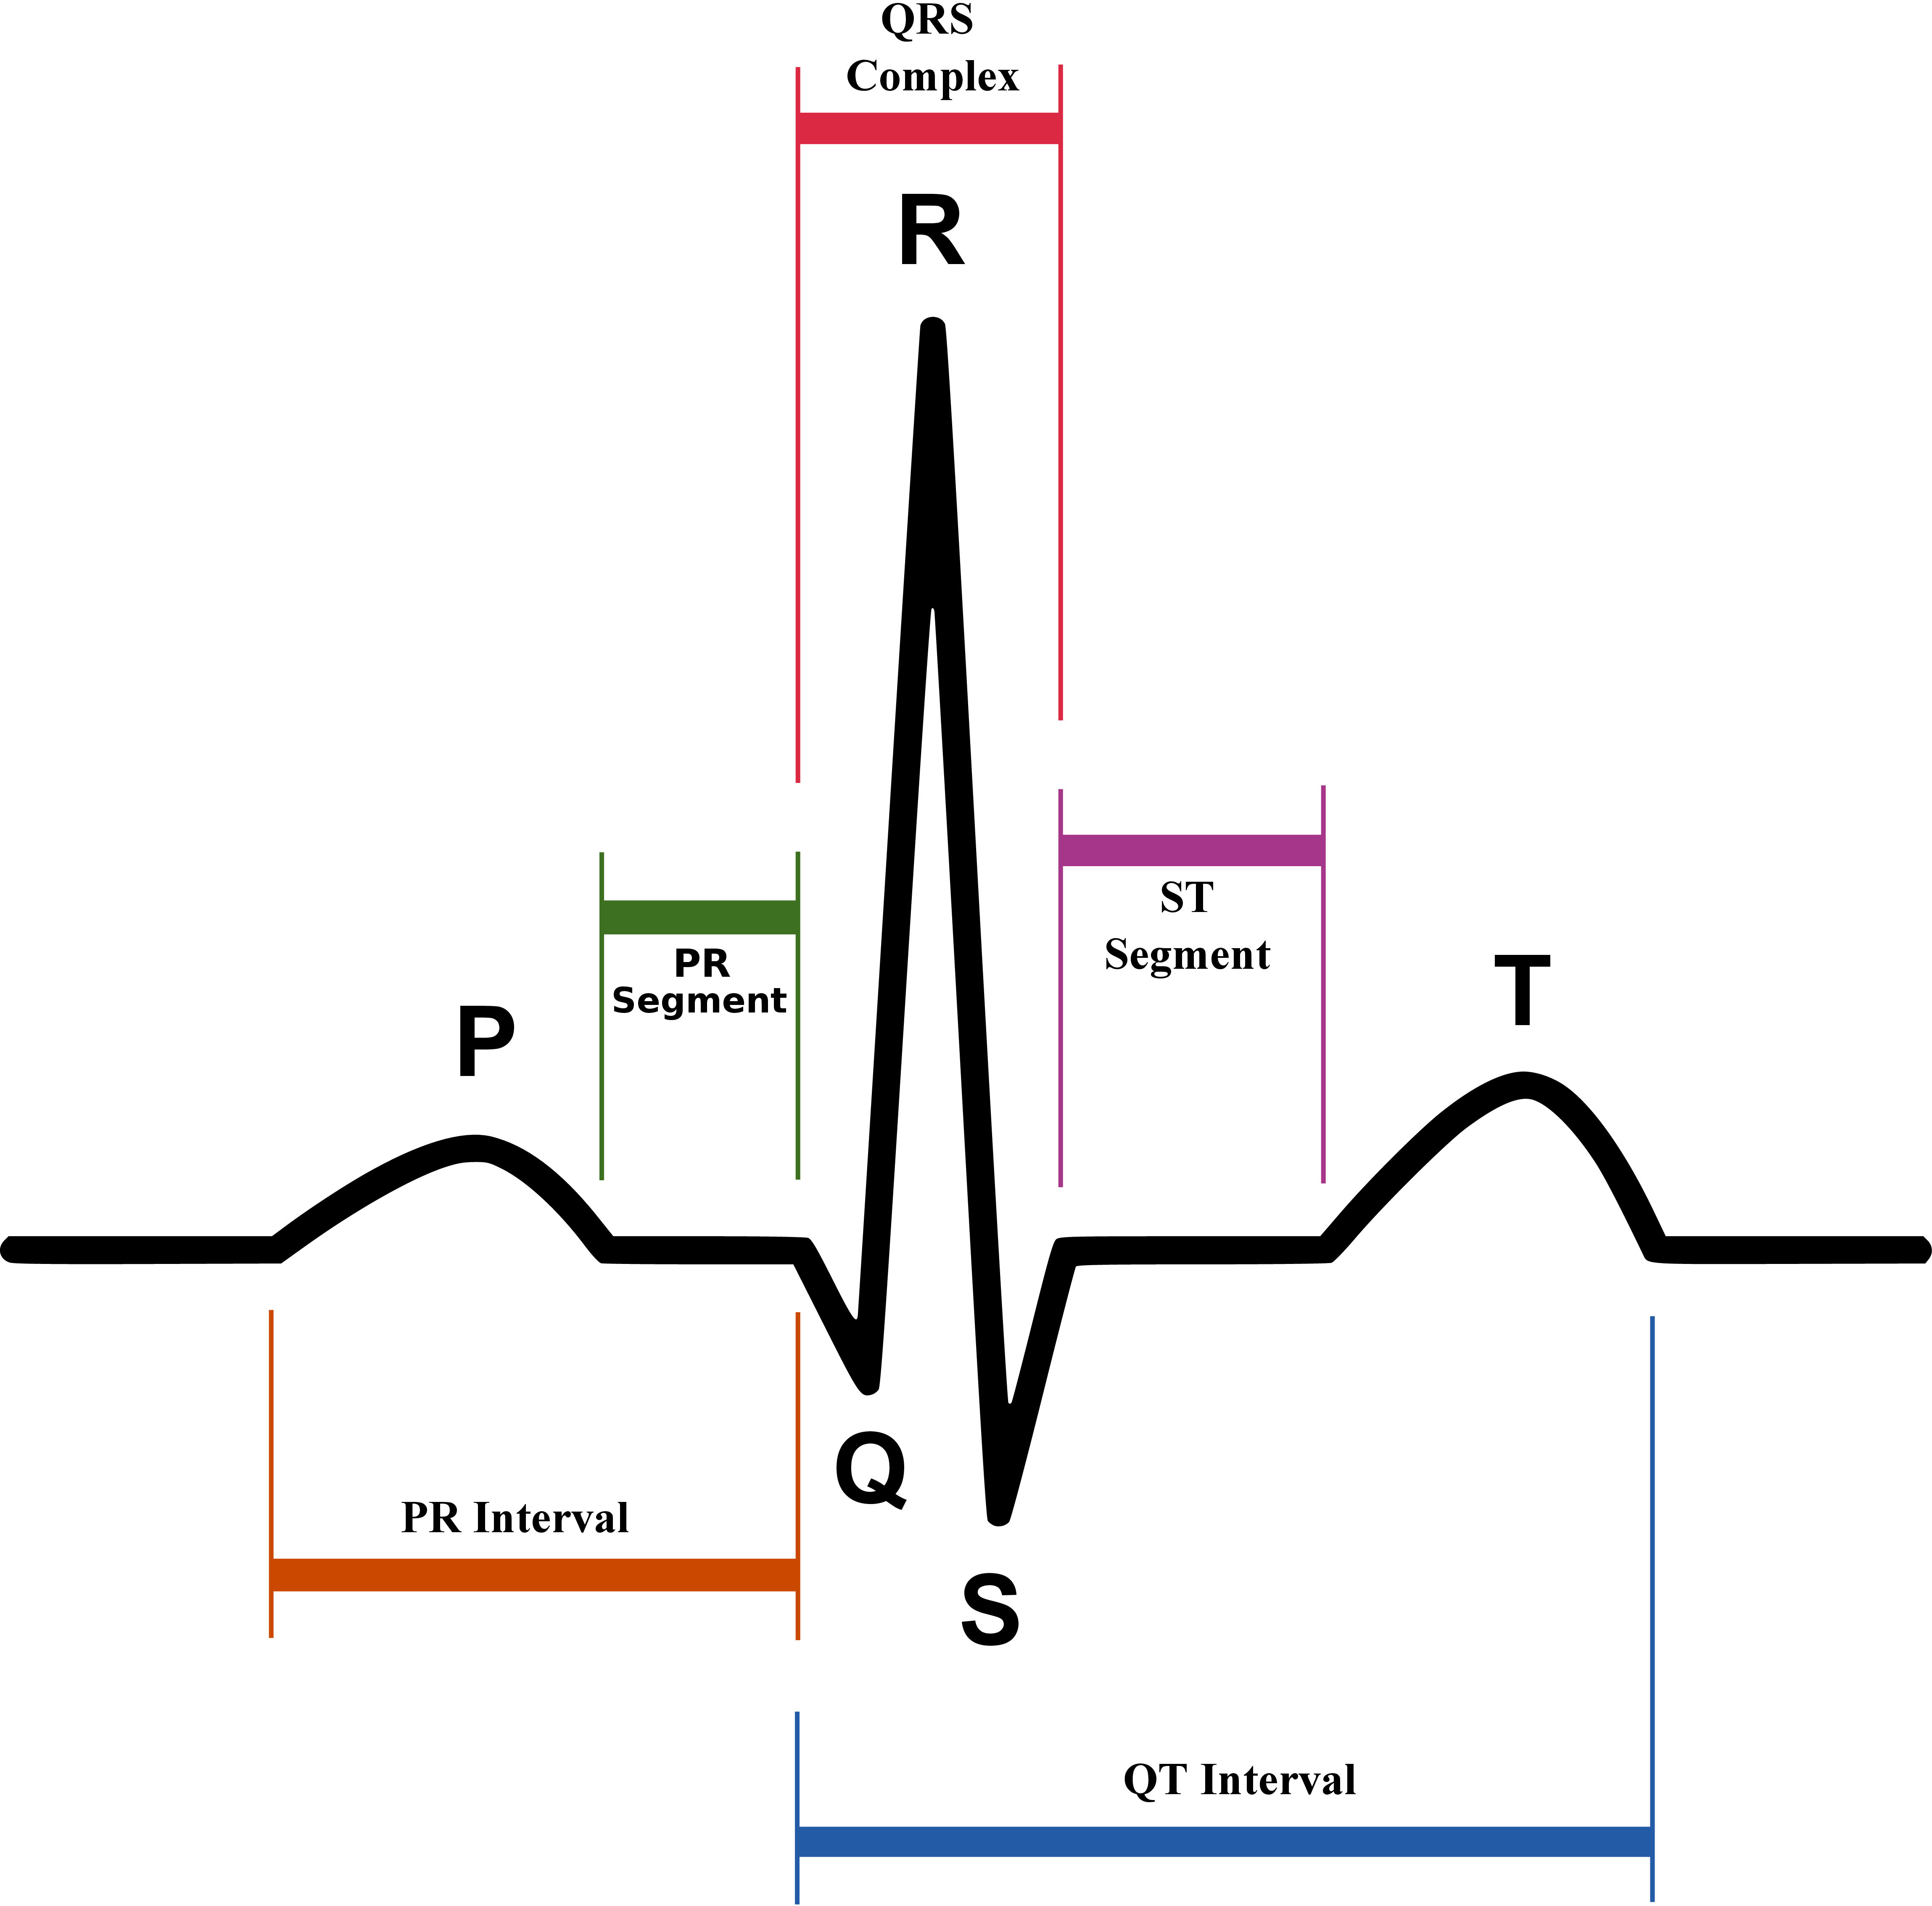
\includegraphics[scale=0.2]{images/SinusRhythmLabels.jpg}
    \caption{A typical ECG wave showing the P wave, QRS complex and S, T waves\cite{wiki:SinusRythmLabels}}
    \label{fig:pqrst}
  \end{figure}

  The P wave represents atrial depolarisation, or the contraction of the two atria.
  The PR interval indicates the time taken for the electrical impulse to reach the ventricles from the atria.
  The QRS complex represents the depolarisation of the ventricles.
  The RT interval denotes the time between depolarisation and repolarization or contraction of the ventricles.
  The T wave, which can be seen as a small wave after the QRS complex, represents ventricular repolarisation.
  The RR interval starts at the peak of one R wave and ends at the peak of the next R wave. It represents the time between two QRS complexes.

  On one hand, low heart rate variability (HRV) has been demonstrated to be a major risk factor leading to various conditions, particularly cardiovascular disorders\cite{kamath1987heart}.
  On the other hand, high HRV has been shown to be an indicator of improved executive functions, such as attentional processing or impulse control\cite{appelhans2006heart, thayer2005psychosomatics}.
  High HRV has also been observed in different psychological conditions associated with symptoms of impaired behavioral and emotional regulation\cite{thayer2009claude, schulz2008negative}.

>>>>>>> upstream/master

  \section{Motivation}
  In recent years, cardiac diseases have drawn great attention as they are the leading cause of mortality in developed countries.
  Long term monitoring of electrocardiogram (ECG) is therefore widely used for those with cardiac ailments.
  Many hardware systems have been proposed for ECG monitoring, which can be differentiated into recording and analyzing systems.

  A typical recording system mainly implements the processes of ECG signal acquisition, storage, and transmission.
  The analyzing system extracts the features from the ECG signal and sends it for analysis.
  Hence, it is necessary to design a joint system for both ECG recording and analyzing of its features, for example, its heart rate variability. Implementing this kind of system involves multiple challenges.
  An energy limited system needs high energy efficiency to prolong its service life.
  In the era of IoT, it is necessary to implement a pocket friendly method which is both portable and convenient.


  \section{Survey of the state of the art}
  % TODO Move technical part of introduction here


  \section{Features we wished to implement}
  % TODO Complete sentences
  Signal acquisition, Pre-processing, extracting features, plotting peaks, HR, Poincare plot


  \newpage
  \section{Our implementation}
  % TODO Add images of our implementation
  \underline{Three sensor pads} are placed on specific regions of the body based on the concept of Einthoven’s triangle\cite{abi2019einthoven}, which is an inverted equilateral triangle as shown in figure \ref{fig:eithoven_triangle}. The voltages at these points give a net potential of zero, making the electrode setup electrically equilateral.

  \begin{figure}
    \centering
    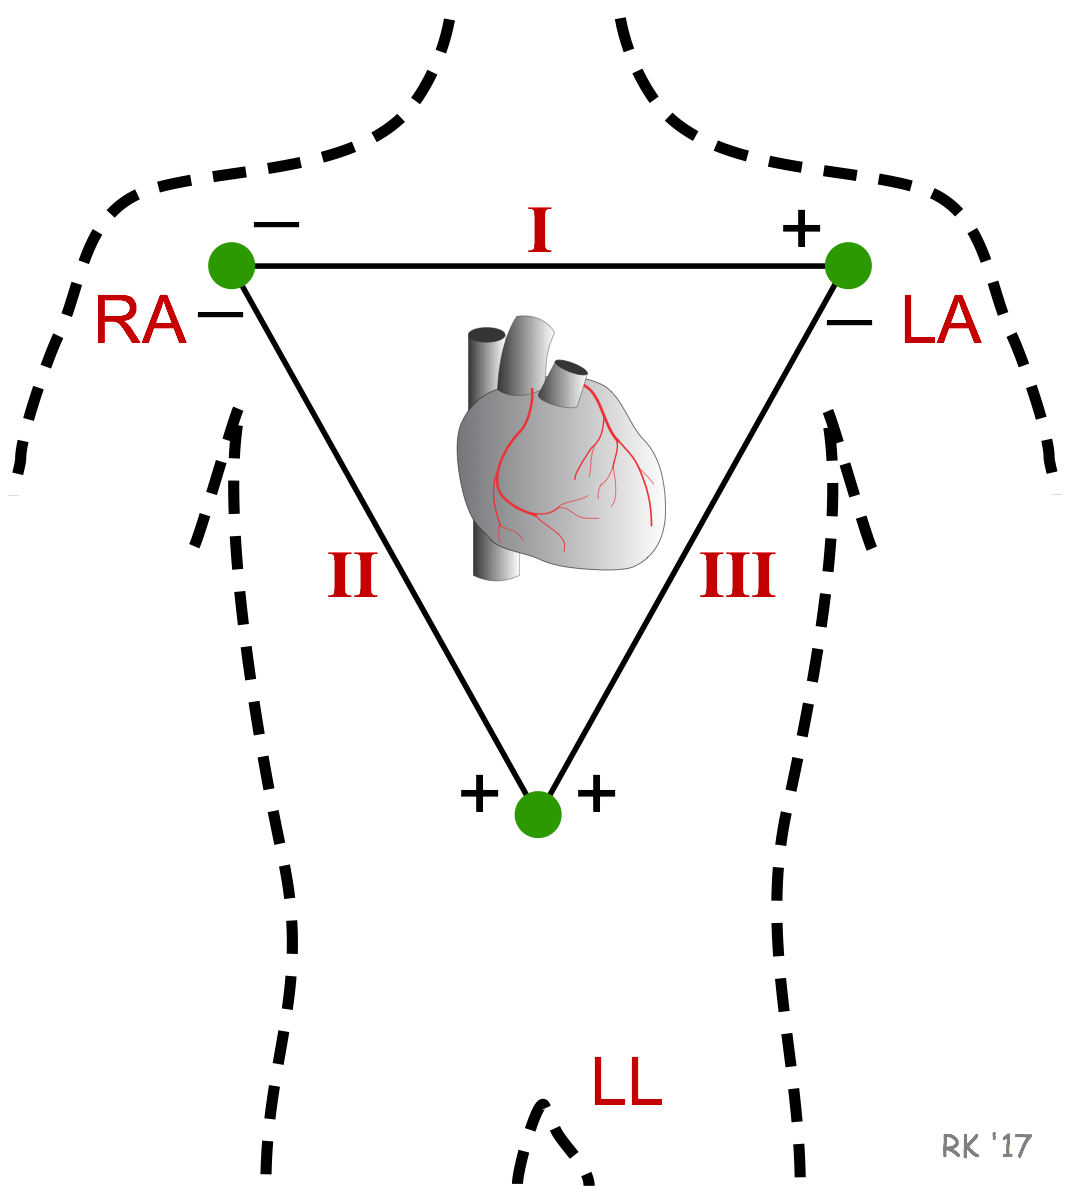
\includegraphics[scale=0.1]{images/eithoven_triangle.png}
    \caption{Eithoven's triangle\cite{cvp:ECG_eithoven}}
    \label{fig:eithoven_triangle}
  \end{figure}

  \underline{AD8232}\cite{ae:ad8232} module which is an integrated signal conditioning block for ECG and other biopotential signals.
  It is designed to extract, amplify, and filter small biopotential signals in the presence of noisy conditions, such as those created by motion or remote electrode placement.
  Its design allows it to be used as a part of low power and low cost applications.
  The AD8232 can implement a two-pole high-pass filter for eliminating motion artifacts.
  After an abrupt signal change that rails the amplifier (such as a leads off condition), the AD8232 automatically adjusts to a higher filter cutoff.
  This feature allows the AD8232 to recover quickly, and therefore, to take valid measurements soon after connecting the electrodes to the subject.


  \underline{Arduino Uno} used to record the data from the AD8232 at a fixed sampling rate.
  The data is then serially transmitted to the Raspberry Pi which can handle more complex processes using more computing power.
  Raspberry Pi 3B+ used to process and analyse the signals.
  Short segments of ECG signals are taken and filtered, smoothened and normalized.
  A Peak detection algorithm is applied and then features are extracted from the RR durations in an ECG signal, where RR represents the period between two consecutive R peaks.
  On the Raspberry Pi, a Jupyter Notebook can be used to provide an interactive environment for signal processing and plotting different waveforms and graphs.
  The peak detection algorithm has been tested on the MAHNOB-HCI\cite{lichtenauer2011mahnob} dataset.

  Features extracted include:
  % TODO Add pictures for each feature
  \begin{itemize}[topsep=1pt]
    \item[] \textit{Mean RR} gives the average value of the RR duration in an ECG segment.
    \item[] \textit{SDNN} is the standard deviation of the NN (R-R) intervals
    \item[] \textit{MSSD} is the root mean square of the successive differences of RR intervals, used for a good snapshot of the Autonomic Nervous System’s Parasympathetic branch and is the basis of the HRV Score.  RMSSD is considered as one of the most relevant and accurate measures of autonomic Nervous system activity over the short-term.
    \item[] \textit{NN50}is the number of pairs of successive NN (R-R) intervals that differ by more than 50 ms
    \item[] \textit{PNN50} is the proportion of NN50 divided by the total number of NN (R-R) intervals
    \item[] \textit{Poincare Plot} is graphed by plotting every R–R interval against the prior interval, creating a scatter plot.
    Poincare plot analysis allows researchers to visually search for patterns buried within a time series.
    The analysis of this plot is a geometrical and nonlinear method to assess the dynamics of HRV.
    The degree of heart failure can be evaluated quantitatively through the computation of the standard deviation (SD) indexes of the plot\cite{hsu2012poincare}.
  \end{itemize}


  \section{Conclusions and Future Work}

  % TODO Complete sentences
  Diagnosis of cardiac and neurological disorders.
  Better sensors give better results
  Data can be sent to the cloud, processed there and then to the app


  \newpage
  \bibliography{bibliography}
  \bibliographystyle{ieeetr}
\end{document}